\section{Основные методы микро- и наноструктурирования}

\subsection{Наноимпринтная литография}
Наноимпринтная литография (НИЛ) -- технология, предназначенная для переноса изображения наноструктуры или электронной схемы на полимерный материал путем прямого воздействия на него специальным штампом~\cite{NIL_1, NIL_2}.
Существуют два основных метода НИЛ -- термическая и ультрафиолетовая (УФ).
В термической НИЛ штамп вдавливается в слой полимера, нагретого до температуры, превышающей температуру стеклования полимера, затем происходит охлаждение полимера и извлечение штампа (рисунок~\ref{fig:NIL}a).
В ультрафиолетовой НИЛ штамп из материала, прозрачного в УФ части спектра, погружается в жидкий полимер, который отверждается под действием УФ излучения, после чего происходит извлечение штампа (рисунок~\ref{fig:NIL}б).
Штампы обычно изготавливается с помощью электронно-лучевой литографии из металла или кремния для термической НИЛ, и из полимеров или кварца -- для УФ НИЛ.
Учитывая прямой контакт штампа с основным материалом, а также масштаб печати 1:1, к плоскопараллельности и бездефектности штампа предъявляются высокие требования.
Перед проведением процесса НИЛ на штамп наносится специальное антиадгезионное покрытие, что позволяет избежать прилипания полимера к штампу при его отделении.
Также после процесса НИЛ на штампе неизбежно остается тонкий остаточный слой полимера, который удаляют с помощью плазменного травления.
Несмотря на то, что технология НИЛ изначально создавалась как альтернатива фото- и электронно-лучевой литографии, она может применяться для получения трехмерных микро- и наноструктур, таких как фотонные кристаллы~\cite{NIL_nanophotonics}, микроканалы~\cite{NIL_microfluidics} и \linebreak др.~\cite{NIL_3D_1, NIL_3D_2}.
Преимуществами НИЛ являются относительная простота процесса (при наличии штампа), высокая производительность и возможность достижения высокого разрешения (менее 100 нм).
К недостаткам этого метода относятся трудоемкость и дороговизна процесса изготовления штампа надлежащего качества, необходимость его частого обслуживания, сложность совмещения штампа с низлежащим слоем и ограниченный ресурс штампа.

\begin{figure}[t]
	\centering
	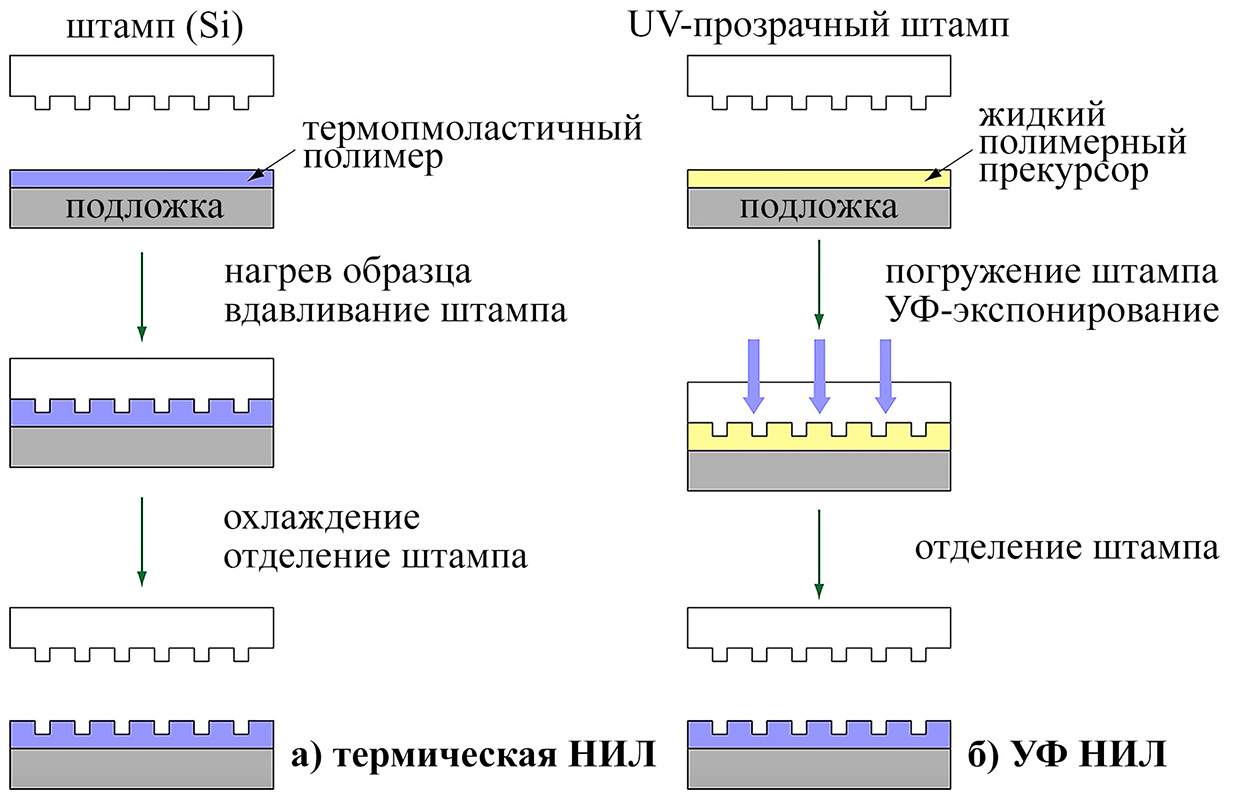
\includegraphics{1_chapter/NIL_14pt_200}
	\vspace{1em}
	\caption{Схематическое изображение метода термической (а) и ультрафиолетовой (б) наноимпринтной литографии.}
	\label{fig:NIL}
\end{figure}


\subsection{Двухфотонная лазерная литография}

Двухфотонная лазерная литография (ДЛЛ) — технология формирования микро- и наноструктур, основанная на двухфотонном поглощении внутри фокального объема лазерного излучения~\cite{Hohmann2015, Kawata2001}. Фотовозбуждение компонент литографической смолы, приводящее к ее отверждению, происходит лишь в окрестности перетяжки сфокусированного лазерного излучения благодаря нелинейному характеру поглощения (рисунок~\ref{fig:TPL}а). Процесс отверждения имеет пороговый характер, что позволяет регулировать размер отверждаемого объема, изменяя дозу или плотность энергии поглощенного лазерного излучения. Последующее погружение смолы в растворитель приводит к удалению тех участков, которые не были подвергнуты воздействию излучения. В качестве источников излучения в ДЛЛ обычно используются фемтосекундные лазеры, работающие в инфракрасном диапазоне, в качестве литографической смолы -- вещество, содержащее реакционно-способные олигомеры и фотоинициатор. При точной фокусировке ДЛЛ способна обеспечить субмикронное разрешение (рисунок~\ref{fig:TPL}б). Поскольку в ДЛЛ положения центров отвреждения могут задаваться произвольно, эта технология нашла применение во многих областях -- микрофлюидике~\cite{TPL_microfluidics_1, TPL_microfluidics_2}, биологии и \linebreak медицине~\cite{TPL_biology_1, TPL_biology_2}, оптике и нанофотонике \cite{TPL_optics, TPL_nanophotonics}, и др. При этом, силу своей природы, данная технология обладает крайне низкой производительностью, что является ее главным недостатком.

\begin{figure}[h]
	\centering
	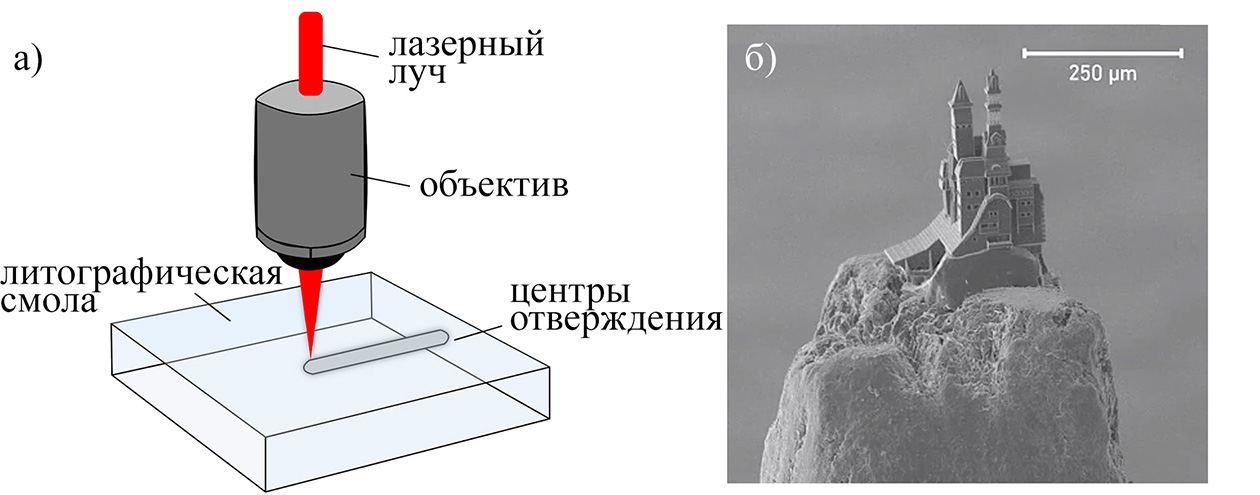
\includegraphics{1_chapter/TPL_14pt_200}
	\vspace{1em}
	\caption{Схематическое изображение метода двухфотонной лазерной литографии (а) и пример структуры, полученной этим методом (б)~\cite{TPL_castle}.}
	\label{fig:TPL}
\end{figure}


\subsection{Интерференционная литография}

Интерференционная литография (ИЛ) -- метод формирования периодической структуры в резисте, основанный на экспонировании резиста пространственно упорядоченным стоячим электромагнитным полем, возникающим при интерференции двух и более когерентных монохроматических или квазимонохроматических пучков излучения~\cite{IL_general} (рисунок~\ref{fig:IL}). Когерентность интерферирующих пучков обычно обеспечивается путем разделения исходного пучка на нужное число вторичных пучков с помощью различных интерференционных схем. В оптическом и УФ-диапазонах используются зеркальные схемы (Френеля, Ллойда и др.), схемы на преломляющей оптике (бипризма Френеля, билинза Бийе) или комбинированные зеркально-линзовые схемы. В этих диапазонах в качестве источника исходного пучка с высокой степенью монохроматичности и когерентности используются лазеры, позволяющие достичь разрешения ИЛ до 100~нм. Вопрос обеспечения более высокого разрешения решается путем перехода в область рентгеновского излучения~\cite{IL_X-ray}. ИЛ применяется для получения  метаматериалов~\cite{IL_metamaterials}, нанофотонных и наноплазмонных устройств~\cite{IL_nanophotonics}, биомедицинских объектов~\cite{IL_biomedical}, изделий на основе выращиваемых наноэлементов и самоорганизующихся структур~\cite{IL_self-assembly} и др. Преимущества метода заключаются в относительной простоте и высокой производительности, к недостаткам можно отнести возможность получения исключительно периодических структур.

\begin{figure}[t]
	\centering
	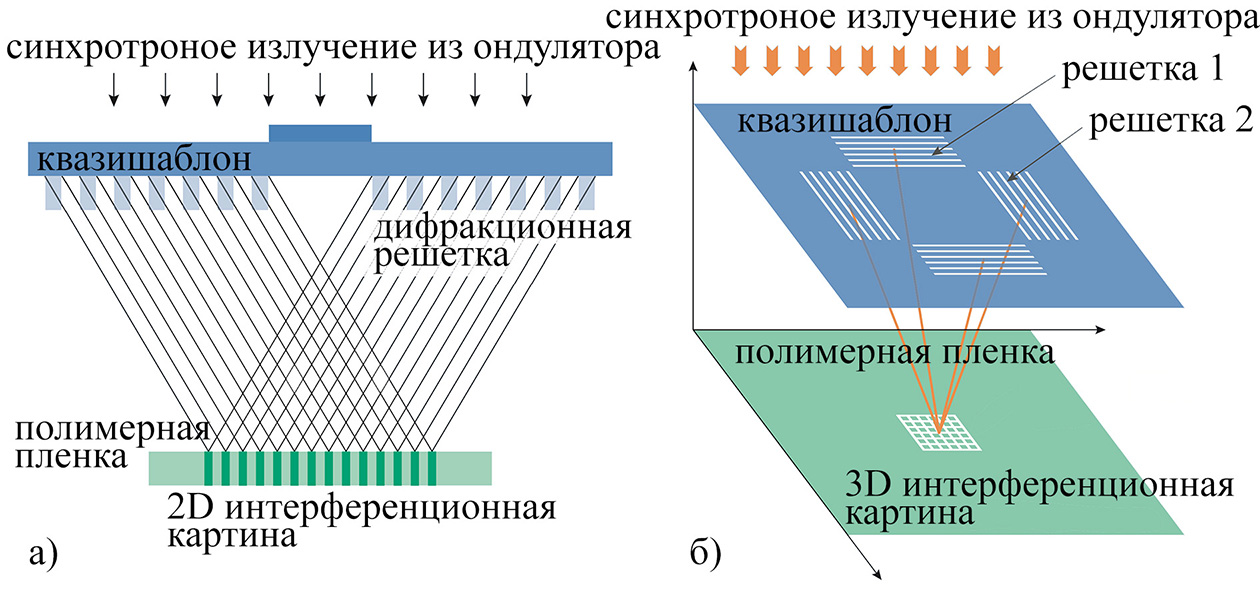
\includegraphics{1_chapter/IL_14pt_200}
	\vspace{0.5em}
	\caption{Схематическое изображение процесса получения двумерных (a) и трехмерных (б) структур методом интерференционной литографии.}
	\label{fig:IL}
\end{figure}


\subsection{Полутоновая литография}

Полутоновая литография (ПЛ) -- общее название для методов, позволяющих получить сложный трехмерный рельеф в литографическом процессе с одной одной стадией экспонирования~\cite{GL_general}. В их основе лежит пространственная модуляция дозы при экспонировании, приводящая к локальному увеличению или уменьшению скорости растворения резиста при проявлении. Таким образом, конечный рельеф, получаемый в резисте, имеет ступенчатую форму и состоит из участков, растворенных в различной степени. Сглаживание границ между участками, проэкспонированных с различными дозами, может быть в дальнейшем достигнуто за счет оплавления образца при температурах вблизи его температуры стеклования (рисунок~\ref{fig:GL}a). При этом такое оплавление может быть использовано как дополнительный этап микроструктурирования~\cite{Kirchner_reflow} (рисунок~\ref{fig:GL}б--г). Таким образом, полутоновая литография с последующим оплавлением образца является гибкой технологией микро- и наноструктурирования, применяемой в оптике и нанофотонике~\cite{GL_optics}, микрофлюидике~\cite{GL_microfluidics}, для формировании микроэлектромеханических систем~\cite{GL_MEMS} и в других областях. Существует как электронно-лучевая, так и фото-ПЛ, однако, фото-ПЛ имеет некоторые ограничения, связанные с оплавлением резиста. Так, например, вязкость широко используемого негативного фоторезиста SU-8 при экспонировании увеличивается, что усложняет процесс его контролируемого оплавления~\cite{Kirchner_GL_review}. Преимущества метода ПЛ заключаются в его универсальности -- варьирование дозы экспонирования и контролируемое оплавление образца позволяют получить практически любой необходимый рельеф. Недостатками метода являются его сложность и производительность, еще более низкая, чем в случае электронно-лучевой литографии.

\begin{figure}[t]
	\centering
	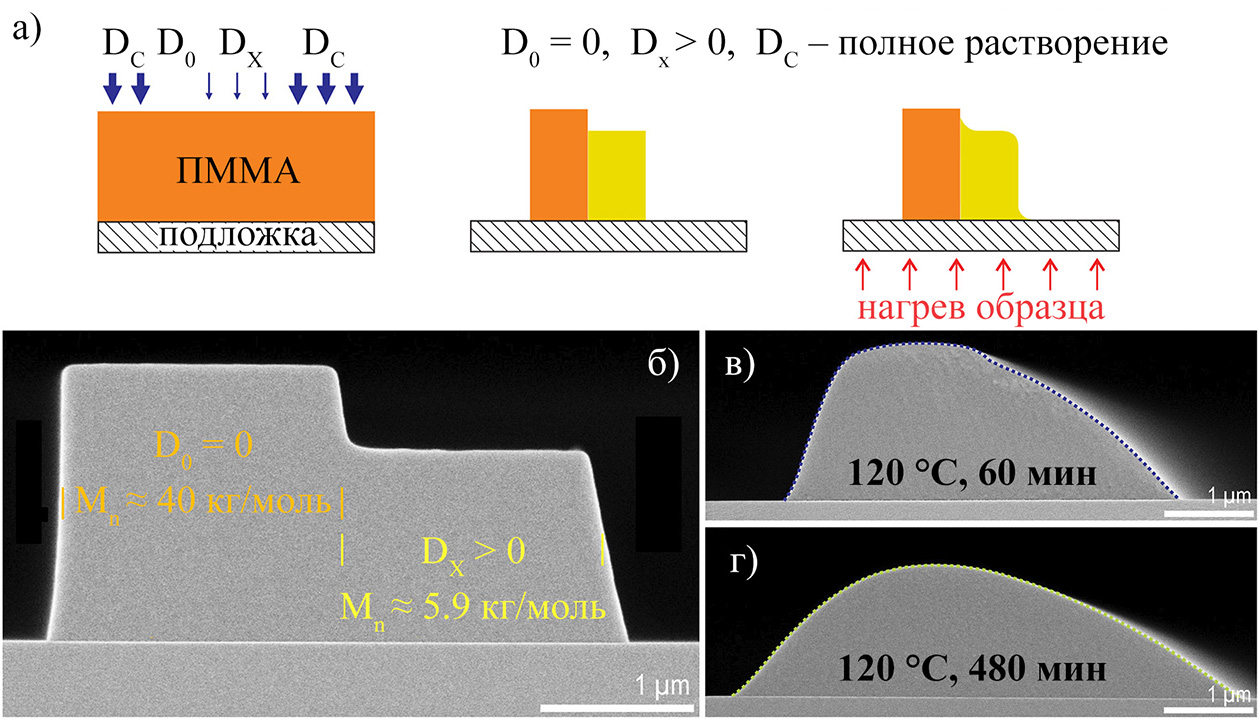
\includegraphics{1_chapter/GL_14pt_200}
	\vspace{1em}
	\caption{Схематическое изображение процесса полутоновой литографии с последующим оплавлением резиста (а) и примеры структуры, полученной в ПММА непосредственно после проявления (б) и при последующем нагреве (в,~г)~\cite{Kirchner_reflow}.}
	\label{fig:GL}
\end{figure}


\subsection{Сканирующая зондовая литография}

Сканирующая зондовая литография (СЗЛ) включает в себя семейство технологий формирования структур с наноразмерным разрешением.
Каждая из технологий основана на применении специального зонда для воздействия на поверхность образца, приводящего к локальным изменениям поверхности.
В зависимости от природы воздействия зонда на поверхность образца можно выделить следующие основные виды СЗЛ:
\begin{itemize}
	\item механическая, в которой изменение поверхности образца происходит в результате механического воздействия зонда~\cite{SPL_mechanical};
	\item  термохимическая, в которой воздействие нагретого зонда на поверхность образца приводит к термической активации различных химических реакций в образце~\cite{SPL_termochemical};
	\item СЗЛ с приложением напряжения, при которой высокая напряженность электростатического поля, создаваемого зондом, приводит к разложению молекул жидкости~\cite{SPL_bias_liquid} или газа~\cite{SPL_bias_gas}, окружающих образец, и локальному отложению материала на образце;
	\item окислительная СЗЛ, основанная на модификации поверхности образца путем ее локального окисления~\cite{SPL_oxidation};
	\item перьевая СЗЛ, в которой сканирующий зонд используется для нанесения на поверхность образца органических, полимерных или коллоидных наночернил~\cite{SPL_dip_pen_1, SPL_dip_pen_2}.
\end{itemize}

Поскольку зонд воздействует только на поверхность образца, этот метод может быть использован только для послойного формирования рельефа (в отличие от, например, ДЛЛ). Однако, высокое разрешение СЗЛ и возможность ее проведения с использованием различных материалов обеспечили ей широкое применение. При этом, как и в случае ДЛЛ, производительность сканирующей зондовой литографии является крайне низкой.


\subsection{Методы на основе термической деполимеризации резиста}

Процесс цепной термической деполимеризации полимерных молекул~\cite{depol_general_1}, обратный процессу полимеризации, может быть использован для формирования рельефа в полимерном резисте.
Цепная термическая деполимеризация резиста может протекать при температурах выше температуры стеклования резиста, и для инициирования этого процесса требуется нарушение целостности главной цепи полимерной молекулы, приводящее к радикализации концов молекулы в месте разрыва~\cite{depol_general_2}.
В процессе цепной термической деполимеризации резиста от полимерной молекулы последовательно отделяется большое число мономеров (по различным данным, от нескольких сотен до нескольких тысяч~\cite{Cowley_1952_1, Mita_PMMA_zip_lengths_T, Inaba_zip_len}), которые вследствие диффузии покидают область, в которой находилась молекула.
Это приводит к появлению свободного пространства в резисте, что и позволяет использовать этот процесс в целях микро- и наноструктурирования.

Существуют два устоявшихся подхода к микроструктурированию на основе цепной термической деполимеризации резиста.
В каждом из них нагревание резиста производится локально, что ограничивает область деполимеризации резиста.
Первый подход по своей сути является термической сканирующей зондовой литографией, в которой для нарушения целостности полимерных молекул используется нагретый зонд~\cite{depol_fabrication_probe}.
Во втором подходе используется сфокусированный лазерный луч, который вызывает локальный нагрев резиста и разрывы в главной цепи его молекул~\cite{depol_fabrication_laser}.

Однако, существует еще один подход, предполагающий нагрев всего слоя резиста, что позволяет цепной реакции термической деполимеризации протекать в любой его области.
На этом подходе основан метод сухого электронно-лучевого травления резиста (СЭЛТР), в котором резист экспонируется электронным лучом при температурах, превышающих температуру стеклования резиста~\cite{Bruk_2016_mee}.
%Отличительными особенностями этого метода является высокая производительность и возможность формирования в резисте дву- и трехмерных структур со скругленным профилем в одностадийном процессе.
%Описанию этого метода будет посвящена вторая часть данной главы.
